\begin{figure}[!htbp]
    \centering
    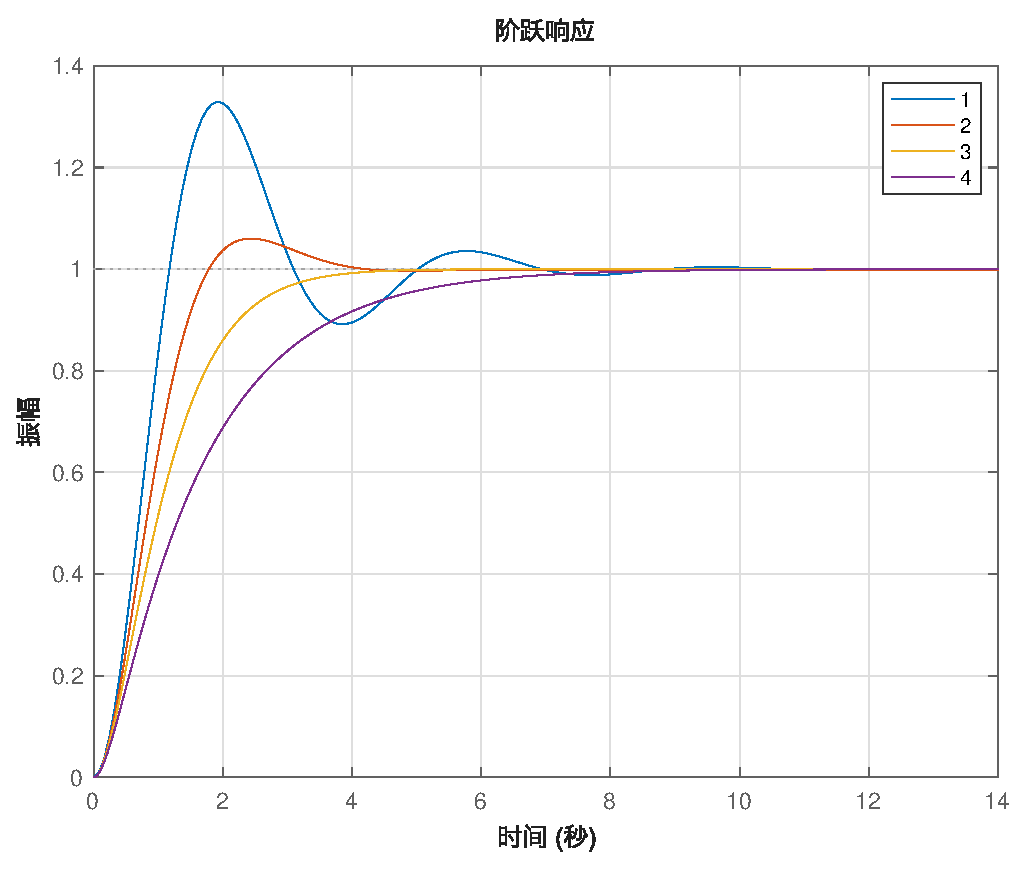
\includegraphics[width=\linewidth]{myplot}
    \caption{...}
\end{figure}

报到地点：成都市高新区（西区）西源大道2006号电子科技大学清水河校区六号科研楼。入选营员在报到时必须携带如下材料：本人身份证（原件）、学生证（原件）、电子科技大学优秀大学生暑期夏令营活动申请表（系统中打印并签字盖章）、夏令营营员入营须知（后续发放）。

2、学生食宿及交通

外地院校学生请自行预定往返车票及住宿。我院为入营学生提供夏令营期间的校内餐食费用补贴，并统一购买在电子科技大学活动期间的团体意外保险。夏令营期间或结束后，学员若在成都有其他安排，不在学院的责任范围内，建议各位营员自行购买旅途意外险。


报到地点：成都市高新区（西区）西源大道2006号电子科技大学清水河校区六号科研楼。入选营员在报到时必须携带如下材料：本人身份证（原件）、学生证（原件）、电子科技大学优秀大学生暑期夏令营活动申请表（系统中打印并签字盖章）、夏令营营员入营须知（后续发放）。

2、学生食宿及交通

外地院校学生请自行预定往返车票及住宿。我院为入营学生提供夏令营期间的校内餐食费用补贴，并统一购买在电子科技大学活动期间的团体意外保险。夏令营期间或结束后，学员若在成都有其他安排，不在学院的责任范围内，建议各位营员自行购买旅途意外险。


报到地点：成都市高新区（西区）西源大道2006号电子科技大学清水河校区六号科研楼。入选营员在报到时必须携带如下材料：本人身份证（原件）、学生证（原件）、电子科技大学优秀大学生暑期夏令营活动申请表（系统中打印并签字盖章）、夏令营营员入营须知（后续发放）。

2、学生食宿及交通

外地院校学生请自行预定往返车票及住宿。我院为入营学生提供夏令营期间的校内餐食费用补贴，并统一购买在电子科技大学活动期间的团体意外保险。夏令营期间或结束后，学员若在成都有其他安排，不在学院的责任范围内，建议各位营员自行购买旅途意外险。


报到地点：成都市高新区（西区）西源大道2006号电子科技大学清水河校区六号科研楼。入选营员在报到时必须携带如下材料：本人身份证（原件）、学生证（原件）、电子科技大学优秀大学生暑期夏令营活动申请表（系统中打印并签字盖章）、夏令营营员入营须知（后续发放）。

2、学生食宿及交通

外地院校学生请自行预定往返车票及住宿。我院为入营学生提供夏令营期间的校内餐食费用补贴，并统一购买在电子科技大学活动期间的团体意外保险。夏令营期间或结束后，学员若在成都有其他安排，不在学院的责任范围内，建议各位营员自行购买旅途意外险。


报到地点：成都市高新区（西区）西源大道2006号电子科技大学清水河校区六号科研楼。入选营员在报到时必须携带如下材料：本人身份证（原件）、学生证（原件）、电子科技大学优秀大学生暑期夏令营活动申请表（系统中打印并签字盖章）、夏令营营员入营须知（后续发放）。

2、学生食宿及交通

外地院校学生请自行预定往返车票及住宿。我院为入营学生提供夏令营期间的校内餐食费用补贴，并统一购买在电子科技大学活动期间的团体意外保险。夏令营期间或结束后，学员若在成都有其他安排，不在学院的责任范围内，建议各位营员自行购买旅途意外险。


报到地点：成都市高新区（西区）西源大道2006号电子科技大学清水河校区六号科研楼。入选营员在报到时必须携带如下材料：本人身份证（原件）、学生证（原件）、电子科技大学优秀大学生暑期夏令营活动申请表（系统中打印并签字盖章）、夏令营营员入营须知（后续发放）。

2、学生食宿及交通

外地院校学生请自行预定往返车票及住宿。我院为入营学生提供夏令营期间的校内餐食费用补贴，并统一购买在电子科技大学活动期间的团体意外保险。夏令营期间或结束后，学员若在成都有其他安排，不在学院的责任范围内，建议各位营员自行购买旅途意外险。


报到地点：成都市高新区（西区）西源大道2006号电子科技大学清水河校区六号科研楼。入选营员在报到时必须携带如下材料：本人身份证（原件）、学生证（原件）、电子科技大学优秀大学生暑期夏令营活动申请表（系统中打印并签字盖章）、夏令营营员入营须知（后续发放）。

2、学生食宿及交通

外地院校学生请自行预定往返车票及住宿。我院为入营学生提供夏令营期间的校内餐食费用补贴，并统一购买在电子科技大学活动期间的团体意外保险。夏令营期间或结束后，学员若在成都有其他安排，不在学院的责任范围内，建议各位营员自行购买旅途意外险。


报到地点：成都市高新区（西区）西源大道2006号电子科技大学清水河校区六号科研楼。入选营员在报到时必须携带如下材料：本人身份证（原件）、学生证（原件）、电子科技大学优秀大学生暑期夏令营活动申请表（系统中打印并签字盖章）、夏令营营员入营须知（后续发放）。

2、学生食宿及交通

外地院校学生请自行预定往返车票及住宿。我院为入营学生提供夏令营期间的校内餐食费用补贴，并统一购买在电子科技大学活动期间的团体意外保险。夏令营期间或结束后，学员若在成都有其他安排，不在学院的责任范围内，建议各位营员自行购买旅途意外险。


报到地点：成都市高新区（西区）西源大道2006号电子科技大学清水河校区六号科研楼。入选营员在报到时必须携带如下材料：本人身份证（原件）、学生证（原件）、电子科技大学优秀大学生暑期夏令营活动申请表（系统中打印并签字盖章）、夏令营营员入营须知（后续发放）。

2、学生食宿及交通

外地院校学生请自行预定往返车票及住宿。我院为入营学生提供夏令营期间的校内餐食费用补贴，并统一购买在电子科技大学活动期间的团体意外保险。夏令营期间或结束后，学员若在成都有其他安排，不在学院的责任范围内，建议各位营员自行购买旅途意外险。
